In \cref{chap:intro_berkovich} the only analytic curves we studied in any detail were the projective line and its affinoid domains like balls and annuli.
Studying these spaces was possible because we had the Berkovich classification  theorem (\cref{thm:berkovich_classification}) which gives an explicit description of the semi-norms on $K[t]$. 
For other varieties, in particular curves it is not as easy to describe all norms.
The solution to this is to understand the relation between models of a variety and its Berkovich analytification. 


In this chapter we cover the theory of weight functions, skeleta and the relation between models of a variety and its analytification described in the papers \cite{mustataWeightFunctionsNonArchimedean2015, nicaiseBerkovichSkeletaBirational2016, bakerWeightFunctionsBerkovich2016}.
We won't do this in full detail, and often restrict ourselves to the case of curves.
This theory works under the assumption that $K$ is discretely valued. 
A similar theory relating models of curves and Berkovich spaces in the case where $K$ is algebraically closed is described in \cite{bakerStructureNonarchimedeanAnalytic2013}. 
While we won't cover this theory, a motivated reader might want to look into it, as it aids our conceptual understanding of Berkovich analytic curves.  

\todo{What to do with the places where Art remarked that the text is subjective.}


\section{Notation} \label{sec:notation}
Let $R$ be a complete discrete valuation ring with fraction field $K$ and algebraically closed residue field $k$. 
The main examples for $K$ to keep in mind are finite extensions of $\C((t)), \hat{\Q_p^{\text{un}}} $ and $\hat{\F_p}((t))$.  
Let $\pi$ be a uniformiser for $R$ and the valuation $v$ on $R$ and $K$ is scaled such that $v(\pi) = 1$. 
The norm on $R$ and $K$ is given by $|x| = \exp(-v(x))$. 

Throughout the chapter we let $X$ be a smooth $K$-variety. 
Any curve will be smooth, proper, geometrically connected, 1-dimensional $K$-variety, usually denoted by $C$. 
If any of these assumptions are not needed in a theory it will be explicitly stated. 

Models are always regular and proper and are usually denoted by script letters like $\mathscr X, \mathscr C$ for $X, C$ respectively.  


In what comes we will mostly study $X\an$ as a topological space together with the analytification map $X\an \to X$. 
To that end we will use the following simpler definition of the Berkovich analytification.

\begin{definition}\label{def:berkovich_analytification_explicit}
	The \emph{Berkovich analitification} of a locally finite type scheme $X$ over  $K$, as a set is \[
		X\an = \{(x, |\cdot |)  \mid x\in X, |\cdot | \text{ a norm on } \kappa(x) \text{ extending the norm on }K \} 
	.\] 

	This comes equipped with a canonical projection map $i: X\an \to X, (x, |\cdot |) \mapsto  x$.
	$X\an $ comes with a topology which we define to be the coarsest topology such that 
	\begin{itemize}
		\item $i: X\an \to X$ is continuous, i.e. $X\an$ is a finer space than  $X$. 
		\item For every open $U \subset X$ and $f \in \mathcal{O}_X(U)$ the map  \[
				|f|: i^{-1}(U) \to \R^{+}: (x, |\cdot |) \mapsto  |f(x)|
		\] 
		is continuous.
	\end{itemize}
\end{definition}
Note that we can still define the completed residue field at a point $x \in X\an$ as \[
	\mathcal{H} ((x, |\cdot |)) = (\kappa(x), |\cdot |)^{\wedge}
.\] 


\section{Different types of points in $X^{\an}$} \label{sec:different_types_of_points_in_xan}
In \cref{sec:types_of_points_in_analytic_curves} we made a distinction between four types of points on the analytification of curves. 
In our context we can also find related but different types of points for varieties over arbitrary dimension. 

\begin{definition}
	The \emph{birational points} of $X\an$ are the points of $X\bir = i ^{-1}(\eta_X)$ where $\eta_X$ is the generic point of $X$. 
\end{definition}
These are called the birational points of $X\an$ because they are shared by the analytification of all varieties birational to $X$.

The opposite of birational points, are the points in the inverse image of a closed points. 
\begin{lemma}
	There is a natural injection \[
		j: X_\text{cl}  \to X\an 
	,\] 
	where $X_\text{cl} $ are the closed points of $X$, such that $i \circ j = \id _{X_\text{cl} }$. 
	We will often implicitly identify points of $X_\text{cl} $ with points in $X\an$. 
\end{lemma}
\begin{proof}
	It is sufficient show that for $x \in X_\text{cl} $, the preimage $i^{-1}(x)$ contains exactly one point. 
	Note that $[\kappa(x):K]$ is finite. 
	Hence there is a unique extension of the norm on $K$ to $\kappa(x)$ (\cref{thm:norm_finite_field_ext}) from which the claim follows. 
\end{proof}

In the \cref{sec:reduction}, we constructed the reduction map $\red_{\mathscr X}: X\an \to \mathscr X$. 
There it was essential to assume that that $\mathscr X$ is proper, in order make sure that any map $\mathcal{H} (x) \to X$ extends to a map $\mathcal{H} ^{o}(x) \to \mathscr X$. 
If $\mathscr X$ is not proper, such an extension does not always exist hence the reduction map is only defined on a subset of $X\an$. 
\begin{definition}
	Given a model $\mathscr X$ of $X$ a point $x \in X\an $ is called a \emph{center} if the map $\mathcal{H} (x) \to X$ extends to $\mathcal{H}^{o} (x) \to \mathscr X$. 
	Note that this is unique by the valuative criterion of seperatedness. 
	We write $\widehat{\mathscr X}_\eta$ for the set of all centers of $X\an$. 
\end{definition}

If $\mathscr X$ is a normal model of $X$ and $\mathscr X_s = \sum_{i \in I} N_i F_i$ be the decomposition of $\mathscr X_s$ in its irreducible parts, and let $e_i$ be the generic point of $F_i$. 
As stated in \cite[thm 2.2.4]{berkovichSpectralTheoryAnalytic2012}, we know that the $e_i$ have unique inverses along the reduction map. 
We call $\red_{\mathscr X}^{-1}(e_i)$ the \emph{divisorial point} associated to $(\mathscr X, F_i)$.
\begin{definition}
	The \emph{set of divisorial points of $X^\mathrm{an}$}, denoted by  $X^{\text{div}}$ is the set of all points that are the inverse of a generic point of irreducible component of a normal model of $X$ under the reduction map. 
\end{definition} 
\begin{definition}
	Let $x \in X^{\text{div}}$ be divisorial point associated to $(\mathscr X, F)$. 
	Then we say that $x$ has \emph{multiplicity} $N(x)$ which is the multiplicity of $F$ in $\mathscr X_s$. 
\end{definition}
\begin{definition}
	If $C$ is a curve and $x$ a divisorial point on $C\an$ corresponding to $(\mathscr C, F)$ then $x$ has \emph{genus} $g(x)$ with is $g(F')$ where $F'$ is the normalisation of $F$. 
	Note that $F'$ is the curve with function field  $\kappa(f)$ where $f$ is the generic point of $F$. 
\end{definition}
Alternatively we can think of divisorial points in the following way. 
If  $\mathscr X$ is normal we know that $\mathcal{O}_{e_i, \mathscr X}$ is a one-dimensional local ring, i.e.\ a discrete valuation ring, where the valuation (up to scaling by a constant $c$) is given by \[
	v_{e_i}\left( f \right)  = c\cdot \ord_{E_i} f
\] 
where $\ord_{E_i} f$ is the multiplicity of $E_i$ in $(f)$. 
As we know that  $\ord_{E_i} \pi = N_i$, choosing $c = \frac{1}{N_i}$ makes it so that $v_{e_i}(\pi) = 1$. 
Hence extending $v_{e_i}$ to $\mathrm{Frac}(\mathcal{O}_{e_i, \mathscr X}) = K(X)$ yields a valuation that extends the valuation on $K$. 
So this gives a point in $X\bir$. 

We find that $X^{\text{div}} \subset X\bir \subset X\an$. 
\begin{lemma}
	The divisorial points $X^{\text{div}}$ are dense in $X\bir$  
\end{lemma}
\begin{proof}
	See \cite[prop.\ 2.4.9]{mustataWeightFunctionsNonArchimedean2015}
\end{proof}

The divisorial points can also be characterized by their valuation without involving models. 
\begin{lemma}\label{lem:char_div_point}
	Let $X\an$ be a $K$-variety of dimension $n$. 
	The divisorial points of $X\an$ are precisely the discrete valuations $v$ on $K(X)$ that extend the valuation on $K$ and such that the $\trdeg [(K(X),v)^{\sim}, k] = n-1$.
	Moreover, the ramification degree of $K$ in $(K(X), v)$ is precisely the multiplicity of $v$ as a divisorial point.  
\end{lemma}
\begin{proof}
	Let $x = (\mathscr X, E)$ be a divisorial point in $X\an$ corresponding to a model $\mathscr X$ with irreducible component $E$ in the special fiber.
	Let $\xi$ be the generic point of $E$. 
	Then $(K(X), v_x)^{\sim} = (\mathcal{O}_{\xi, \mathscr X})^{\sim} = K(E)$ and hence the transcendence degree is $\dim E = n-1$.

	The converse is given by \cite[lem 2.45]{kollarBirationalGeometryAlgebraic1998}. 
\end{proof}

\begin{remark}
	 If $C$ is a curve, then the divisorial points in $C\an$ are precisely the type $2$ points. 
\end{remark}
\begin{proof}
	This is a consequence of \cref{def:type_points_curve} and \cref{lem:char_div_point}.
	Let $x$ be a birational point and $v_x$ the corresponding valuation on $K(X)$.
	Then $\trdeg[(K(X),x)^{\sim} ] = n-1 = 1 $ if and only if $F_{\mathcal{H} (x) / k} = 1$.
	Also $v_x$ is discrete if and only if $E_{\mathcal{H} (x) / k}= 0$. 
\end{proof}


\begin{remark}
	From \cref{lem:char_div_point} we see that the divisorial points are inherent to the analytic space $X\an$. 
	I.e.\ we do not need models of $X$ to describe the divisorial points. 
	As the value group and residue field of a DVR do not change under completion we also see that the multiplicity and genus in the case of curves are inherent. 
	Indeed for a divisorial $N(x)$ is the ramification degree of $\mathcal{H} (x)$ over $K$ and $g(x)$ is the genus of the curve with function field $\widetilde{\mathcal{H} (x)}$. 
\end{remark}

In the theory we will distinguish one more type of point, will be the content of the next section.


\section{The skeleton of a of a model of a curve} \label{sec:the_dual_graph_of_a_model_of_a_curve}
In the previous section we saw that given a regular model $\mathscr X$ of $X$, we can find divisorial points in $X\an$ that correspond to the irreducible components on the special fibre.  
Moreover, if $\mathscr X$ is an snc-model, then we can find interpolations of these divisorial points along these intersections. 
These will be the \emph{monomial points}. 
We will sketch the construction of these monomial points and why they are useful in the context of curves. 

\subsection{The dual graph of a model of a curve} \label{sec:the_dual_graph_of_a_model_of_a_curve}
\begin{definition}
	Let $\mathscr C$ be a snc-model of a curve $C$.
	Let $F_1, \ldots, F_r$ be the irreducible components in the special fibre, occurring with multiplicity $N_1, \ldots, N_r$ respectively. 
	Then the \emph{dual graph of $\mathscr C$}, written $\Delta(\mathscr C)$, is the graph with vertices $V = \{F_i\}_{i = 1}^{r} $ and the edges between $F_i, F_j$ are the intersection points of $F_i$ with $F_j$. 
\end{definition}
As the model is snc, the intersection number in an intersection point is  $1$. 
So if $i \ne j$ then $F_i$ and $F_j$ are connected by $F_i \cdot F_j$ edges in $\Delta(\mathscr C)$. 
\begin{example}\label{ex:first_dual_graph}
	\begin{enumerate}
		\item Consider an elliptic curve $E$ over $K$ of reduction type $\mathrm I_2$ and let $\mathscr E$ be the minimal snc-model, which incidentally is the same as the minimal regular model. 
			Then the dual graph $\Delta(\mathscr E)$ consists of two points and two edges between them.
		\item Let $\mathscr P$ be the model of $\pro_K^{1}$ from \cref{ex:first_model}. 
			The dual graph consists of two points connected by one edge.  
		\item Let $E'$ be again an elliptic curve, this time of reduction type $\mathrm I_3^*$. 
			And let $\mathscr E'$ be its minimal regular model (which is snc). 
			Then the dual graph has the shape of an H. See \cref{fig:example_dual_graph}.

	\end{enumerate}
\end{example}

\begin{figure}[h]
    \centering
    \incfig{example-dual-graph}
    \caption{The models and dual graphs from \cref{ex:first_dual_graph}}
    \label{fig:example_dual_graph}
\end{figure}

We can equip the dual graph $\Delta(\mathscr C) $ with extra information. 
To every vertex (i.e.\ irreducible component  $F$ of $\mathscr C_s$) we attach the pair $(N(F), g(F))$ consisting of the multiplicity of $F$ and in $\mathscr C_s$ and the genus of $F$ as a $k$-curve with reduced scheme structure. 
So in the third example in \cref{fig:example_dual_graph} the points $G_1, \ldots, G_4$ would be labelled with $(1, 0)$ and $F_1, \ldots, F_4$ with $(2, 0)$. 

We can add even more structure to $\Delta(\mathscr C)$ in the form of a metric. 
\begin{definition}
Let $e$ be an edge connecting $F_i, F_j$, which are irreducible components of multiplicity $N_i, N_j$ respectively. 
Then we define the \emph{length of $e$ }  \[
	\ell(e) = \frac{1}{\lcm (N_i, N_j)}
.\] 
\end{definition}

This allows us to turn $\Delta(\mathscr C)$ into into a metric space by having the vertices $v_i$ be points and for every edge  $e$ connecting $v_i, v_j$ we glue the interval $[0, \ell(e)]$ (a metric space of length $\ell(e)$) along the end points to $v_i, v_j$. 
The metric on $\Delta(\mathscr C)$ is then given by the shortest path metric. 
So $\Delta(\mathscr E )$ from \cref{fig:example_dual_graph} would be a circle of length 2 and $\Delta (\mathscr P)$ a line of length $1$. 
But the line connecting $F_1, F_2$ in $\Delta(\mathscr E')$ would only be $1 /2$ long. 
\begin{definition}
	The metric/topological space described above is written as $|\Delta(\mathscr C)|$. 
\end{definition}

\subsection{The skeleton: embedding the dual graph into $C^{\mathrm{an}}$}\label{sec:skeleton}
The following theorem is the main reason why snc-models are useful when studying Berkovich geometry. 
\begin{theorem}
	Let $\mathscr C$ be a snc-model of a curve $C$. 
	Then there is a natural embedding \[
		\sk_{\mathscr C}:|\Delta(\mathscr C)| \into \mathscr C\an
	,\]
	such that for any irreducible component $F$ of $\mathscr C_s$,  $\sk_{\mathscr C}(F)$ is the divisorial point associated to $F$. 
\end{theorem}
\begin{proof}
	A rigorous proof can be found in \cite[3.1.4]{mustataWeightFunctionsNonArchimedean2015}.
	We will give a sketch of the argument. 
	Let $\mathscr C = \sum_{i= 1}^{r} N_i F_i$ be the decomposition into irreducible components. 
	We know what the images of the vertices $F_1, \ldots, F_r$ of $\Delta(\mathscr C)$ must be.
	What is missing is the map on the edges. 

	Let $e$ be an edge connecting vertices $F_i, F_j$. 
	Recall that $e$ corresponds to an intersection $\xi \in \mathscr C_s$ that belongs to both to $F_i$ and $F_j$. 
	The idea is construct a family of norms/valuations on $\mathscr \mathcal{O}_{\xi, \mathscr C}$ that interpolate between the divisorial points associated to $F_i, F_j$. Then we can extend these norms the faction field $K(C)$. 

	Let $t_i, t_j$ be local equations cutting out $F_i, F_j$ in a neighbourhood of  $\xi$. 
	Then $t_i, t_j$ are a regular system generating the maximal ideal of $\mathcal{O}_{\xi, \mathscr C}. $ 
	They satisfy \[
		t_i ^{N_i} t _j^{N_j} = u\cdot \pi
	\] 
	where $u$ is unit in $\mathcal{O}_{\xi, \mathscr C}$, as $\pi$ (the uniformaiser) cuts out $F_i, F_j$ with multiplicity $N_i, N_j$ respectively.  
	Let $0 \le \alpha_i \le 1 / N_i,   0 \le \alpha_j \le 1 / N_j$ be real numbers such that \begin{equation}\label{eq:barycentic_alphas}
		N_i\cdot \alpha_i + N_j \cdot \alpha_j = 1
	.\end{equation}
	
	Now we can define a norm on $\mathcal{O}_{\xi, \mathscr C}$. 
	Let  $f$ be any function in $\mathcal{O}_{\xi, \mathscr C}$. 
	Considering $f$ as a element in the completion $\hat{\mathcal{O}_{\xi, \mathscr C}}$ we can write $f$ as power series expansion in $t_i, t_j$  \[
		f = \sum_{\ell, m}^{} a_{\ell, m} t_i ^{\ell} t_j^{m}
	.\] 
	On this power series we can define a valuation similar to the valuation we defined  for affinoid algebras as \[
		v_{\alpha_i, \alpha_j}(f) = \inf_{\alpha_{\ell, m} \ne 0}{\alpha_i \ell + \alpha_j m}
	.\] 
	One can show that this does not depend the chosen power series expansion and that it is a well defined valuation. 
	As we required \eqref{eq:barycentic_alphas} we have that  $v_{\alpha_i, \alpha_j}(\pi) = 1$ so this valuation extends the valuation on $K$. 
\end{proof}
\begin{definition}
	Let $\mathscr C$ be a snc-model of a curve $C$. 
	Then the \emph{skeleton} associated to $\mathscr C$ is the image of the of the embedding $|\Delta(\mathscr C)|$ in $C\an$. 
	\[
		\sk(\mathscr C) = \im \sk_{\mathscr C}
	.\] 
\end{definition}
\begin{definition}
	The points that are in the skeleton $\sk(\mathscr)$ of some snc-model $\mathscr C$ are called \emph{monomial points}. 
	The set of monomial points in $C\an$ is written as  $C^{\text{mon}}$. 
\end{definition}

So our different types of points have the following relations \[
C^{\text{div}} \subset C^{\text{mon}} \subset C\bir \subset C\an \supset C_\text{cl}
.\] 

\begin{remark}
	It is possible to generalize this construction to higher dimensional varieties. 
	The dual graph has to be replaced by a dual complex and the monomial points must interpolate between more divisorial points along a simplex.
	This is worked out in detail in \cite{mustataWeightFunctionsNonArchimedean2015}. 
	However, we will only need the theory for curves. 
\end{remark}
\todo[inline]{example of skeleta, mostly elliptic curves}


\subsection{Dual graphs, skeleta and blowups} \label{sec:dual_graphs_and_blowups}
We can study how the dual graphs of models behave under blowing up the points of the special fibre.
Essentially this is translating \cref{lem:blowup_snc} to the language of dual graphs.
Let $x$ be a closed point in the special fibre, $\mathscr C' = \bl_{x} \mathscr C$ the blowup, and $E$ be the exceptional divisor in $\mathscr C'$.

We first consider what happens if $x $ is a smooth point of $\mathscr C_s$. 
Let $F$ be the irreducible component of $\mathscr C_s$ that contains $x$ and let $N$ be the multiplicity of $F$. 
Then $E$ is a rational curve of multiplicity $N$, which only intersects $\tilde F$ in one point. 
The strict transforms of the components in $\mathscr C$ all intersects each other in the same way in $\mathscr C'$. 
So in the dual graph we have to add one vertex $E$ labelled $(N, 0)$ (multiplicity and genus) which is connected to $F$ by one edge.

There are two natural maps between $|\Delta(\mathscr C)|$ and $|\Delta(\mathscr C')|$. 
\[
\begin{tikzcd}
	{|\Delta(\mathscr C')|} \rar[hookleftarrow, shift left]{i} \rar[twoheadrightarrow, shift right, ']{r} & {|\Delta(\mathscr C)|} 
\end{tikzcd}
.\] 
An isometric inclusion $i$ and a deformation retraction $r$ that retracts the edge between  $E$ and $F$. 
Note that $r \circ i = \id_{|\Delta(\mathscr C)|}$ and that the maps are a homotopy equivalence. 
See \cref{fig:blowup_smooth_point_skeleton}. 

\begin{figure}[ht]
    \centering
    \incfig{blowup-smooth-point-skeleton}
    \caption{The dual graph after blowing up in a smooth point on the special fibre of an snc-model. }
    \label{fig:blowup_smooth_point_skeleton}
\end{figure}

\begin{remark}
	Blowing up $ F$ in another point $x'$ results in an extra edge on the dual graph. 
	Embedding this in $C\an$, this edge lays in another tangent direction at$F$ in $C\an$. 
	So we see that every closed point  on  $F$ gives a tangent direction at the divisorial point $F$. 
	With the theorem we see later, we see that conversely every tangent direction also corresponds to a closed point on $F$. 
	This is illustrated in \cref{fig:blowup_smooth_point_skeleton}.
\end{remark}


\medskip

We now consider what happens if $x$ is an intersection point of $\mathscr C$. 
Let $F, G$ be the components that contain $x$, of multiplicity $M, N$ respectively. 
Then the strict transforms $\tilde F, \tilde G$ no longer intersect in $x$, but they both intersect the exceptional divisor $E$ in one point. 
Recall that $E$ is a rational curve of multiplicity $M + N$ (\cref{lem:blowup_snc}). 
So in the dual graph $\Delta(\mathscr C')$ the edge $e$ between $F, G$ corresponding to $x$ is replaced by an edge $e_1$, from $F$ to $E$ and an edge $e_2$ from $E$ to $G$. 
Note that \[
	\ell(e) = \frac{1}{\lcm(M, N)} = \frac{1}{\lcm(M, M + N)} + \frac{1}{\lcm(M+ N, N)} = \ell(e_1) + \ell(e_2)
.\]  
So in the dual graph we have put an extra vertex on the edge $e$, turning it into two edges, while keeping the total length the same.
See \cref{fig:blowup_intersection_points_skeleton}. 
So again we find an isometry $i$ and a retraction $r$
\[
\begin{tikzcd}
	{|\Delta(\mathscr C')|} \rar[hookleftarrow, shift left]{i} \rar[twoheadrightarrow, shift right, ']{r} & {|\Delta(\mathscr C)|} 
\end{tikzcd}
.\] 
In this case the retraction is just the inverse as $i$ is actually an isomorphism. 

\begin{figure}[ht]
    \centering
    \incfig{blowup-intersection-poins-skeleton}
    \caption{The dual graph after blowing up in an intersection point on the special fibre of an snc-model. }
    \label{fig:blowup_intersection_points_skeleton}
\end{figure}

Now let $f:\mathscr C' \to \mathscr C$ be any dominating map between snc-models of $C$. 
By the factorisation theorem \cref{thm:factorisation_theorem} we find that $f$ can be decomposed by a sequence of blowups in closed points. 
\[
\mathscr C' = \mathscr C_n \to \mathscr C_{n-1} \to \ldots \to \mathscr C_0 = \mathscr C
.\] 
With corresponding isometric inclusions and retractions 
\[
\begin{tikzcd}
	{|\Delta(\mathscr C_{j})|} \rar[hookleftarrow, shift left]{i_j} \rar[twoheadrightarrow, shift right, ']{r_j} & {|\Delta(\mathscr C_{j-1})|} 
\end{tikzcd}
.\] 
Composing these inclusions and retractions we find the following proposition
\begin{proposition}\label{prop:inclusion_retraction_dual_graph}
	Let $f:\mathscr C' \to \mathscr C$ be any dominating map between snc-models of a curve $C$. 
	Then there is a natural isometric inclusion $i$ and deformation retraction $r$
\[
\begin{tikzcd}
	{|\Delta(\mathscr C')|} \rar[hookleftarrow, shift left]{i} \rar[twoheadrightarrow, shift right, ']{r} & {|\Delta(\mathscr C)|} 
\end{tikzcd}
,\] 
	which are homotopy equivalences
\end{proposition}

The inclusion $i: |\Delta(\mathscr C)| \into |\Delta(\mathscr C')|$ is compatible with the embedding into $C\an$, which we make precise in the following theorem. 
\begin{proposition}
	Let $f:\mathscr C' \to \mathscr C$ be any dominating map between snc-models of a curve $C$ and $i$ the inclusion $i: |\Delta(\mathscr C)| \into |\Delta(\mathscr C')|$. 
	Then the following diagram commutes \[
	\begin{tikzcd}
		& C\an \\
		{|\Delta(\mathscr C)|} \ar[hookrightarrow]{ur}{\sk_{\mathscr C}}
\ar[hookrightarrow]{rr}{i} & & {|\Delta(\mathscr C')|} \ar[hookrightarrow]{ul}[']{\sk_{\mathscr C'}}
	\end{tikzcd}
	.\] 
	In particular there is an inclusion of skeleta $\sk(\mathscr C) \subset  \sk(\mathscr C')$, which is compatible with the metrics and $\sk(\mathscr C)$ is a deformation retract of  $\sk(\mathscr C')$. 
\end{proposition}

By the previous proposition all the results we have about $|\Delta(\mathscr C)|$ actually also work with  $\sk(\mathscr C)$. 
\todo{this is not very precise language}

\begin{corollary}
	Let $C$ be a curve with  $g(C) > 0$, $\mathscr C$ any snc-model of $C$ and $\mathscr C_\text{min} $ the minimal snc-model. 
	Then there is an isometric inclusion $i$ and deformation retraction $r$
\[
\begin{tikzcd}
	\sk(\mathscr C ) \rar[hookleftarrow, shift left]{i} \rar[twoheadrightarrow, shift right, ']{r} & \sk(\mathscr C_\text{min} ) 
\end{tikzcd}
.\] 
In particular $\sk(\mathscr C_\text{min} )$ has the same homotopy type as every other skeleton of $C$. 
\end{corollary}
\begin{proof}
	This is \cref{prop:inclusion_retraction_dual_graph} together with \cref{thm:minimal_snc_model}.
\end{proof}

\subsection{Skeleta span $C^{\mathrm{an}}$} \label{sec:skeleta_span_C_an}

In the previous sections we have seen that snc-models of $C$ give pieces (skeleta) of $C\an$. 
If we want to use these models to understand the geometry of $C\an$ it is desirable that we can obtain all or most of $C\an$ by looking at skeleta. 
This is the case and is made precise in the following proposition. 
\begin{proposition}\label{prop:skeleta_curve_limits}
	Let $C$ be a curve. Then 
	\begin{align*}
		\mathbb H(C) &= \bigcup_{\mathscr C \text{ snc-model}} \sk(\mathscr C) \\
		C\an &= \varprojlim_{\mathscr C \text{ snc-model}} \sk(\mathscr C)
	,\end{align*}
	where $\mathbb{H}(C)$ as a set are the type 2 and 3 points of $C\an$ and the projective limit is taken over the ordered system of snc-models of $C$ and the maps are the deformations retractions from \cref{prop:inclusion_retraction_dual_graph}.
\end{proposition}
\begin{proof}
	See \cite[§2.2.2 and  lem.\ 2.3.2]{bakerWeightFunctionsBerkovich2016}
\end{proof}
\begin{remark}
	While $\mathbb{H}(C)$ and $C\an$ are almost the same set, their topologies are different. 
	The difference comes down to the following. 
	Let $x$ be a branch point (i.e.\ divisorial/type 2 point).
	Then a neighbourhood $U \subset C\an$ of $x$ must entirely contain all but finitely many branches, whereas a neighbourhood $V \subset \mathbb{H}(C)$ must just be an open when restricted to any skeleton $\sk(\mathscr C)$ (a finite graph). 
\end{remark}

The union in \cref{prop:skeleta_curve_limits} is actually a injective limit over the same ordered system of snc-models, but the maps here are the inclusions. 
As these inclusions are isometries, the metrics on the skeleta $\sk(\mathscr C)$ induce a metric on $\mathbb{H}(C)$, which is called the \emph{stable metric}. 

\begin{remark}
	The \emph{stable metric} is not the only metric on $\mathbb{H}(C)$. 
	In \cite{bakerWeightFunctionsBerkovich2016} they define another but similar metric, the \emph{potential metric} which seems to be better suited to some applications. 
\end{remark}

\begin{remark}
	The stable metric does not generalize to analytification of higher dimensional varieties. 
	On a 1-dimensional topological space, a path metric is equivalent to giving a measure. 
	So saying that $\mathbb{H}(C)$ is a metric space is slightly misleading as it is in fact the measure that generalises to higher dimensions. 
\end{remark}

Let $C$ be a curve and $\mathscr C$ be a snc-model of $C$. 
As $C\an$ is a filtered limit of spaces which when large enough retract to $\sk(\mathscr C)$ (\cref{prop:skeleta_curve_limits,prop:inclusion_retraction_dual_graph}), the following theorem is believable, albeit not entirely trivial to prove. 
\begin{proposition}\label{prop:retract_analytification_skeleton}
	Let $\mathscr C$ be a snc-model of a curve $C$. 
	Then there is a deformation retract $\rho_{\mathscr C}: C\an \to \sk(\mathscr C)$. 
	\question{is this actually a deformation retraction, or just a retraction? 
	It must be a deformation retract, otherwise the inclusion would not be a homotopy equivalence. }
\end{proposition}
\begin{proof}
	See \cite[§2.2.2]{bakerWeightFunctionsBerkovich2016}.
\end{proof}

The metric induces a piecewise affine linear structure on $\mathbb{H}(C)$. 
\begin{definition}
	Let $f: \mathbb{H}(C) \to \R$ be a function. 
	Then $f$ is \emph{piecewise linear} if $f \circ \ell$  is a piecewise linear function for every line $\ell: [a, b] \into \mathbb{H}(C)$ parametrised by length. 

	We say that $f$ is \emph{$\Z$-affine linear} (resp.\ \emph{$\Q$-affine linear}) if moreover the slopes $f \circ \ell$ are in $\Z $ (resp.\ $\Q$)
\end{definition}






\section{Weight functions and the essential skeleton} \label{sec:weight_functions}
We might ask ourselves what a good notion for a minimal skeleton might be. 
A wish list of good properties for such a skeleton $\sk(X)$ is the following. 
\begin{itemize}
	\item The minimal skeleton needs to capture all information about the ``shape'' of $X\an$. 
		This means that the inclusion $\sk(X) \into X\an$ is a homotopy equivalence and it has to contain all all divisorial points whose associated minimal component is not rational.
	\item $\sk(X)$ is canonical. 
	\item $\sk(X)$ is well behaved under (nice) base change. 
\end{itemize}
For a curve $C$ of positive genus there is a canonical minimal skeleton $\sk(\mathscr C_\text{min} )$, with $\mathscr C_\text{min} $ the minimal snc-model.
However, this does not generalize to higher dimensions as not every variety has a minimal snc-model. 
Another drawback is that $\sk(\mathscr C_\text{min})$ is not functorial under base change. 

In \cite{mustataWeightFunctionsNonArchimedean2015} M.\ Mustaţă and J.\ Nicaise construct what they call the \emph{essential skeleton}.
It is defined for any variety with a semi-ample canonical line bundle, which is a much larger class of varieties than those with minimal snc-models. 
In particular, this includes every curve of non-zero genus. 
The essential skeleton is canonical, contains the shape of $X\an$ in the sense of the first wish and it pulls back under tame base-change. 
As we will see at the end of this section is even has some nice properties under some finite morphisms between curves. 
The main tool in defining it are weight functions. 

\subsection{Weight functions} \label{sec:weight_functions}
Given a variety $X$, a weight function is a piecewise $\Z$-affine linear function corresponding to a rational section $\sigma$ of the canonical line bundle. 
They are an important tool to study skeleta because if $\sigma$ is a regular section then the associated weight function $\wt_\sigma$ is strictly increasing away from every skeleton associated to a snc-model. 
So the minimal locus $\minloc \wt_\sigma$ has to be contained in every skeleton of $X$. 
This gives us a way of identifying pieces of a skeleton. 
Taking all these pieces together is the essential skeleton. 
We will only work in the context of curves. 
\nomenclature[minloc]{$\minloc f$}{The minimal locus of the function $f$}

\begin{definition}\label{def:log_cannonical_bundle}
	Let  $\mathscr C$ be a normal proper model of a curve $C $. 
	We define the \emph{log-canonical bundle of $\mathscr C$} to be \[
		\omega_{\mathscr C}^{\text{log}}  = \omega_{\mathscr C / R}(\mathscr C_{s, \text{red}} - \mathscr C_s)
	,\] 
	where $\omega_{\mathscr C}$ is the canonical bundle of $\mathscr C$ and $\mathscr C_{s, \text{red}}$ is the divisor on $\mathscr C$ that contains every irreducible component of $\mathscr C_s$ with multiplicity $1$.  
\end{definition}
\nomenclature[log]{$\omega^{\text{log}}_{\mathscr C}$}{The log-canonical bundle on $\mathscr C$}

Note that the restriction of $\omega_{\mathscr C}^{\text{log}}$ to the generic fiber is the canonical bundle on $C$. 

\begin{remark}
	The log-canonical bundle is actually the analogue of the canonical bundle for log schemes. 
	In this case the $\mathscr C$ has a log structure induced by the special fiber. 
	But for our purposes we can work with the explicit definition above. 
\end{remark}
\begin{definition}
	Let $C $ be a curve.
	The \emph{$m$-pluricanonical line bundle} is the $n$-th tensor power of the ordinary canonical line bundle, $\omega_{C / K}^{\otimes m }$. 
	A \emph{$m$-pluricanonical form}  is a non-zero global section of $\omega_{C / K}^{\otimes m }$. 
	A \emph{$m$-pluricanonical section} is a non-zero rational section of $\omega_{C / K}^{\otimes m }$.
\end{definition}
\nomenclature[mp]{$\omega_{C / K}^{\otimes m }$}{The $m$-pluricanonical linebundle on $C$}
\begin{notation}
	Let $D$ be a Cartier divisor on a scheme $X$, and let $F$ be a prime divisor on $D$. 
	Then we write $\mult_{F}(D)$ for the coefficient of $F$ in $D$. 
\end{notation}

We first define the weight function on a divisorial point and then use a sort of expansion by continuity to define it on the whole of $C\an$. 
\begin{definition}\label{def:weight_function_divisorial_point}
	Let $C$ and $\sigma$ be rational section of $\omega_{C / K}^{\otimes m}$.
	Let $x$ be a divisorial point in $C\an$ and $\mathscr C$ be a regular model  with a irreducible component $F$ of multiplicity $N$ corresponding to $x$. 
	Let $\sigma'$ be the unique extension of $\sigma$ to a $m$-pluricanonical section. 
	Then we define the \emph{weight of $\sigma$ at $x$} to be \[
		\wt_\sigma(x) = \frac{\mult_F(\divisor(\sigma'))}{N}
	.\] 
\end{definition}
\nomenclature[wt]{$\wt_{\sigma}$}{The weight function of the pluricanonical section $\sigma$ on $X$}

\begin{remark}
	If one does not like to work with the log-canonical bundle, we can use an alternative definition that puts a minor error term in the definition of the weight. 
	Let $\sigma"$ be the extension of $\sigma$ to $\omega_{\mathscr C / R}^{\otimes m}$. Then \[
		\wt_{\sigma} = \frac{\mult_F(\divisor (\sigma")) + m}{N} - m
	.\] 
\end{remark}
One can prove that this definition is independent of the model $\mathscr C$ chosen. 
We extend the weight function to $\mathbb{H}(C)$ as follows.
\begin{definition}\label{def:weight_function}
	Let $C$ be a curve and $\sigma$ a rational section of $\omega_{C / K}^{\otimes m}$. 
	Then we define the \emph{weight function} $\wt_{\sigma}: \mathbb{H}(C) \to \R$ to be the unique function such that 
	\begin{itemize}
		\item The restriction $\wt_{\sigma}|_{\sk(\mathscr C)}$ is continuous with respect to the metric topology on $\sk(\mathscr C)$ for any snc-model $\mathscr C$, 
		\item on divisorial points $x$ the value of $\wt_{\sigma}(x)$ agrees with \cref{def:weight_function_divisorial_point}.
	\end{itemize}
\end{definition}

The weight function can even be extended to the entirety of $C\an$, but then it may take $\pm \infty$ as values on the type 1 points. See \cite[§4.5.4]{mustataWeightFunctionsNonArchimedean2015}


Various tools and techniques for computing weight functions on curves can be found in \cite{bakerWeightFunctionsBerkovich2016}. 
These will be useful in \cref{chap:a_berkovich_approach_to_classifying_elliptic_curves}. 

\subsection{The essential skeleton $\sk(C)$}\label{sec:the_essential_skeleton_sk_c$}

Weight functions are interesting for studying models because when $\sigma$ is a $m$-pluricanonical form, i.e.\ a non-zero global section, then $\wt_\sigma$ is strictly increasing away from any skeleton associated to a snc-model. 
This is made precise in the following theorem. 
\begin{proposition}\label{prop:weight_function_increase}
	Let $\mathscr C$ be a snc-model of a curve $C$ and $\sigma$ be $m$-pluricanonical form on $C$ (i.e.\ a global section).
	Let $\rho_{\mathscr C}: C\an \to \sk(\mathscr C)$ be the retract from \cref{prop:retract_analytification_skeleton}. 
	Let $x \in C\an $ be any point. 
	Then \[
		\wt_\sigma(x) \ge \wt_\sigma(\rho_{\mathscr C}(x))
	,\] 
	with equality if and only if $x \in \sk(\mathscr C)$. 
\end{proposition}
\begin{proof}
	See \cite[prop.\ 4.4.4]{mustataWeightFunctionsNonArchimedean2015}. 
\end{proof}

\begin{definition}[Kontsevich–Soibelman skeleton]\label{def:KS_skeleton}
	Let $\mathscr C $ be curve and $\sigma$ a rational pluricanonical form. 
	Then we define the \emph{Kontsevich-Soibelman skeleton of $\sigma$} to be \[
		\sk(C, \sigma) = \minloc \wt_{\sigma}
	.\]  
	Here $\minloc f$ (the minimal locus) is the set where the function $f$ attains its infimum.
\end{definition}
\nomenclature[skcw]{$\sk(C, \sigma)$}{The Kontsevich-Soibelman skeleton on $C$ of $\sigma$}
\begin{lemma}
	Let $\sigma$ be a $m$-pluricanonical form and $\mathscr C$ a snc-model of $C$. 
	Then $\sk(C, \sigma) \subset  \sk(\mathscr C)$
\end{lemma}
\begin{proof}
	This follows from \cref{prop:weight_function_increase}, and the definition of the Kontsevich-Soibelman skeleton. 
\end{proof}
Calling the Kontsevich-Soibelman skeleton a skeleton might be slightly misleading as it might not have the same homotopy type as $C\an$. 
Note that for general $\sigma$ it might even be that $\sk(C, \sigma)$ is empty. 
But if $\sigma$ is a form then $\sk(C, \sigma)$ may be computed on $\sk (\mathscr C)$ for any snc-model $C$ by \cref{prop:weight_function_increase}. 
As $\sk(\mathscr C)$ is compact we know that $\wt_{\sigma}$ attains its minimum on $\sk(\mathscr C)$ and thus $\sk(C, \sigma)$ is non-empty. 
In fact $\sk(C, \sigma)$ will always be the union of edges in $\sk(\mathscr C)$. 
Still $\sk(C, \sigma)$ might only be a small part $\sk(\mathscr C)$. 

The solution to this is to take the union of many Kontsevich-Soibelman skeleta.
\begin{definition}[essential skeleton]
	Let $C$ be a curve. 
	Then the \emph{essential skeleton of $C$} is \[
		\sk(C) = \bigcup_{\sigma} \sk(C, \sigma)
	\] 
	where $\sigma$ runs over all $m$-pluricanonical forms of $C$ for all $m > 1$. 
\end{definition}
\nomenclature[sk]{$\sk(C)$}{The essential skeleton of $C$}
\begin{remark}\label{rem:sufficiently_divisible_pluriconanonical}
	Note that in the definition of the essential skeleton, it is sufficient to let $\sigma$ range over all $m$-pluricanonical forms with $m$ sufficiently divisible. 
	This is because if $\sigma$ is a $m$-pluricanonical form, then $\sigma^{\otimes d}$ is a $md$-pluricanonical form and $\wt_{\sigma{\otimes d}} = d\cdot \wt_{\sigma}$. 
	So $\sk(C, \sigma) = \sk(C, \sigma^{\otimes d})$. 
\end{remark}
\begin{remark}
	While weight functions are defined for \emph{rational sections} of the pluricanonical line bundle $\omega_{C / K}^{\otimes m}$, when we define the essential skeleton we consider the weight functions where $\sigma$ is a \emph{form}, i.e.\ a global section of $\omega_{C / K} ^{\otimes m}$. 
	So it is important to make the distinction between \emph{rational sections} and \emph{forms}.
\end{remark}

It is not at all clear from the definition that the essential skeleton actually captures the shape of $C\an$, i.e.\ has the same homotopy type and contains all the points of non-zero genus. 
If $C = \pro^{1}_K$ then $\sk(C)$ is empty because there are no pluricanonical sections. Indeed the $m$-th pluricanonical line bundle is isomorphic to  $\mathcal{O}(-2m)$, which does not have global sections. 
But for curves of non-zero genus the canonical line bundle is semi-ample and thus $\sk(C)$ is non-zero. 

If $C$ is a curve of genus $g(C) > 0$ then there is a way of obtaining $\sk(C)$ from $\sk(\mathscr C_\text{min} )$, where $\mathscr C _\text{min}$ is the minimal regular model and removing some superfluous tails or rational curves.  

\begin{definition}
	Let $\mathscr C$ be a snc-model for a curve $C$. 
	An irreducible component $F$ of $\mathscr C_s$ (vertex in $\Delta(\mathscr C)$) is called \emph{inessesential}, if in the dual graph it belongs to a path of vertices $v_1, \ldots, v_n$ of genus $0$ with the valency $v(v_1) = 1$, $v(v_{2}) = 2, \ldots, v(v_{n-1}) = 2, v(v_n) > 2$ and $F \ne v_n$. 
	Conversely a component/vertex if called \emph{essential} if it is not inessential. 
\end{definition}
See \cref{fig:inessential_components} for some examples of the essential and inessential vertices on a dual graph. 

\begin{figure}[h]
    \centering
    \incfig{inessential-components}
    \caption{Some hypothetical dual graphs with the inessential components colored red. 
    The numbers next to the vertices are the genus of that component if it differs form zero.}
    \label{fig:inessential_components}
\end{figure}

\begin{theorem}
	Let $C$ be a curve with genus $g(C) > 0$ and let $\mathscr C_\text{min} $ be the minimal snc-model of $C$. 
	Let $\Delta'$ be the complete subgraph of $\Delta(\mathscr C_\text{min} )$ with the essential vertices. 
	Then the essential skeleton is the image of $|\Delta'|$\[
		\sk(C) = \sk_{\mathscr C_\text{min} }(|\Delta'|)
	.\] 
\end{theorem}
\begin{proof}
	The proof is insightful as to obtain this result one needs to understand the relation between weight functions and the pluricanonical forms.
	Unfortunately it is too long to put in this thesis. 
	The interested reader is encouraged to look at \cite[thm 3.3.13]{bakerWeightFunctionsBerkovich2016}. 
\end{proof}
\begin{figure}[h]
	\centering
	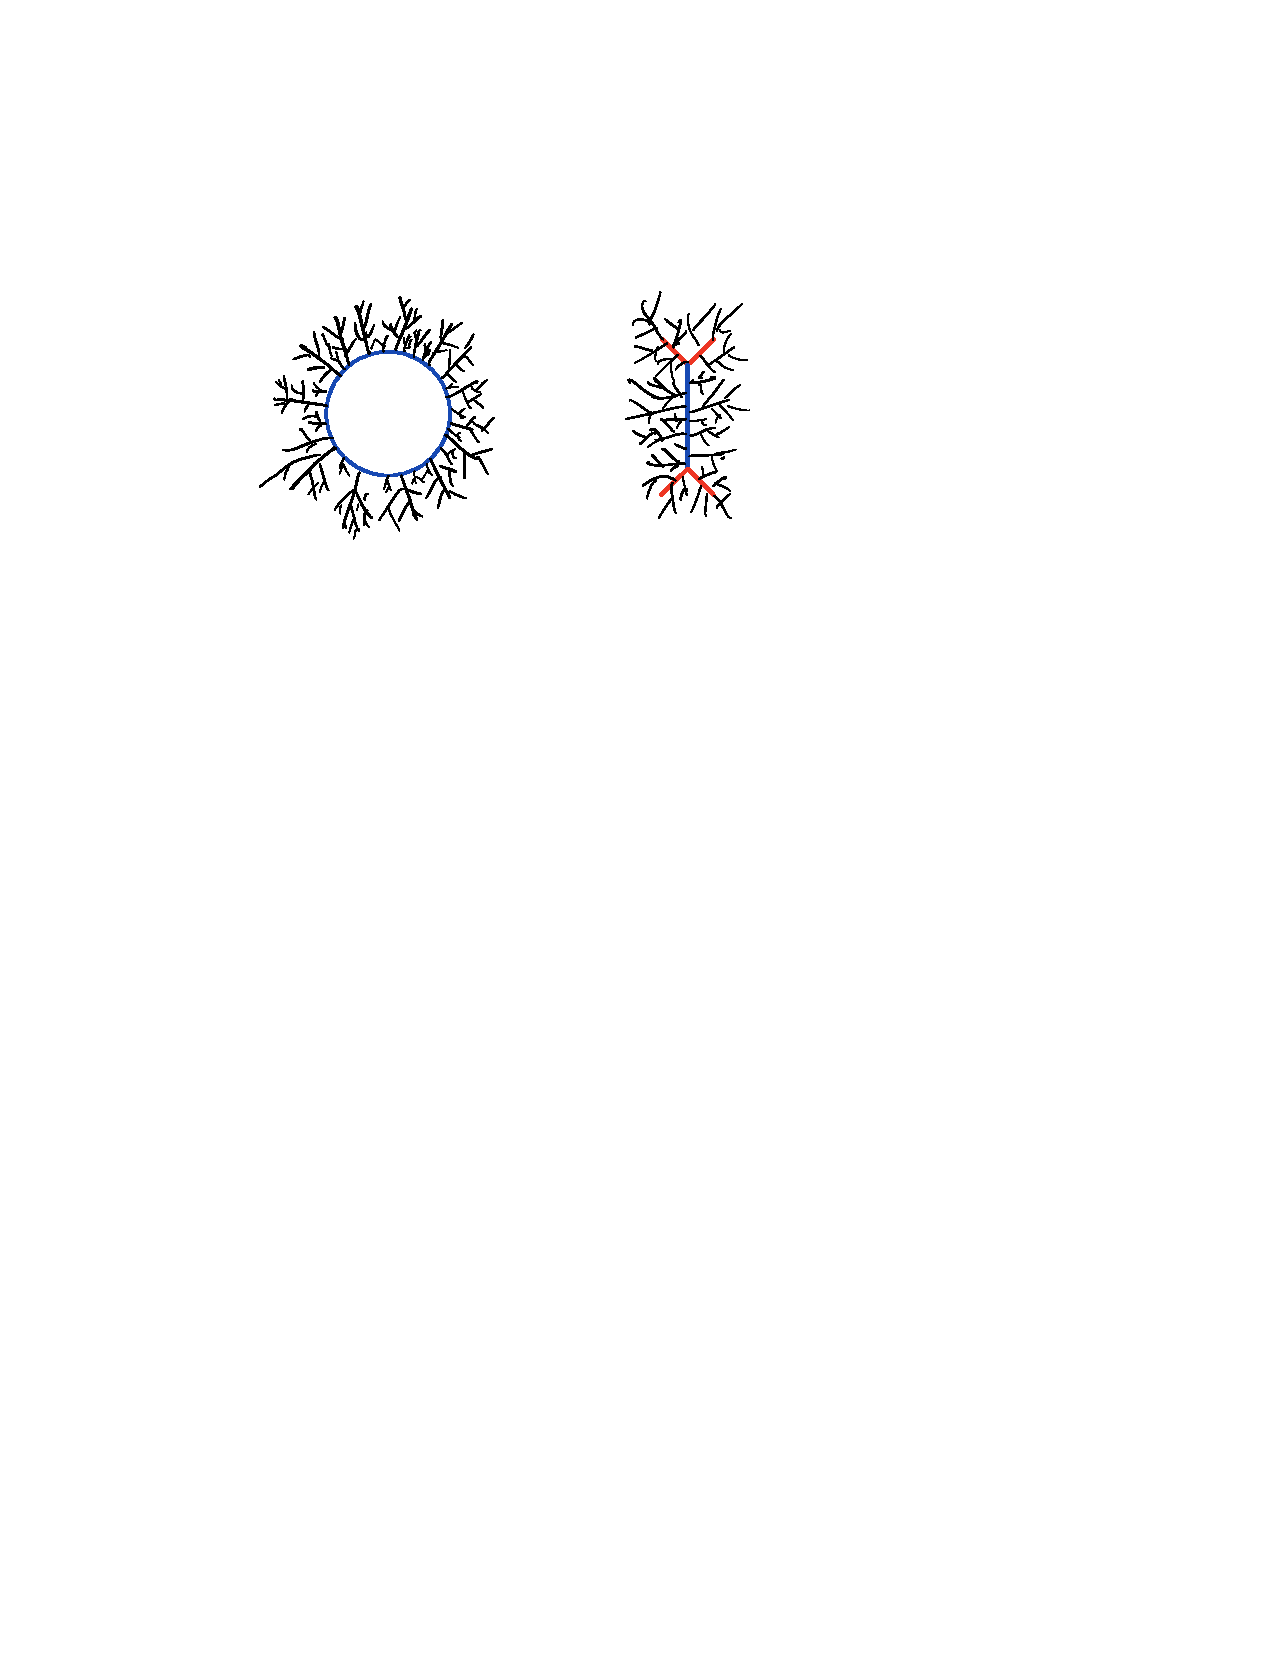
\includegraphics[width=0.6\textwidth]{chapters/weight/figures/essential_skeleton_elliptic.pdf}
	\caption{Artistic renderings of the analytification of an elliptic curve of type $\mathrm I_n, n \ge 1$ (left) and $\mathrm I_n^*, n \ge 1$ (right) with the essential skeleton in blue and the inessential bits of  $\sk(\mathscr E_\text{min} )$ in red. }
	\label{fig:}
\end{figure}



\section{Weight functions and morphisms} \label{sec:weight_functions_and_morphisms}
In this section we study how weight functions behave under morphisms, in particular finite covers of curves. 
The main result of this section, \cref{prop:weightfunction_fullback}, was already known to experts, but it is not stated in the papers we are following \cite{bakerWeightFunctionsBerkovich2016,nicaiseBerkovichSkeletaBirational2016,mustataWeightFunctionsNonArchimedean2015}, and is as far as we know not published elsewhere. 

We first need a few results on the analytification of finite maps between varieties. 

\begin{lemma}
	Let $f: X \to Y$ be a finite map between varieties over  $K$. 
Then the map $f\an: X\an \to Y\an$ is finite. 
\end{lemma}
\begin{proof}
	Let $(y, v) \in Y\an$ with $y \in Y$ and $v$ a valuation on $\kappa(y)$ as in \cref{def:berkovich_analytification_explicit_chap_6}. 
	Then \[
		{f\an}^{-1} (y, v) = \{(x, v_x) \st f(x) = y, v_x \text{ is valuation on $\kappa(x)$ that extends $v$ }  \} 
	.\]
	The number of $x \in X$ such that $f(x) = y$ is finite. 
	For any such $x$ the number of valuations on $\kappa(x)$ that extend $v$ is finite because of \cref{lem:normalisation_extension_norm} and the fact that normalisations of Nagata schemes are finite (\stacks{0335}).
\end{proof}

\begin{lemma}\label{lem:im_type_ii}
	If $f: X \to Y$ is a generically finite map between $K$-varieties and $x \in X^{\text{bir}}$. Then
	\[
		x \in X^\text{div} \iff f(x) \in Y^\text{div}
	.\] 
\end{lemma}
\begin{proof}
	The map being generically finite means that $K(X)$ is a finite extension of $K(Y)$ and that $v_{f(x)}$ is the restriction of $v_x$ to $K(Y)$. 
	Then the residue fields of $K(X), K(Y)$ wrt.\ $v_x, v_{f(x)}$ are a finite extension \stacks{09E5}, hence of the same transcendence degree over $k$. 
	The claim now follows from \cref{lem:char_div_point}.
\end{proof}
\begin{lemma}
	Let $f: X \to Y$ be a finite map and $x \in X^{\text{div}}$, $y = f(x)$, 
	then \[
		N(x) = N(y)\cdot e
	,\]
	where $e$ is the ramification degree of $\mathcal{H} (y) \to \mathcal{H} (x)$. 
\end{lemma}
\begin{proof}
	This is \cref{lem:multiplicative_ramification_degree} applied to the morphisms $\mathcal{H} (y) \to \mathcal{H} (x) \to K$.
\end{proof}
\begin{remark}
	In the case of curves we can give a more topological argument for \cref{lem:im_type_ii}. 
	A divisorial point $x \in X\an$ is precisely a point with an infinite number of tangent directions, i.e.\ a branch point.
	The map $f\an: X\an \to Y\an $ is topologically finite.
	So there are also infinitely many branches at $f(x)$, i.e.\ $f(x)$ is also such a branch point, hence divisorial. 	
\end{remark}

The following proposition will be very useful for understanding finite maps between Berkovich curves in general. 
\begin{proposition}\label{prop:balancing_finite_morphism}
	Let $g: X \to Y$ be a generically finite map between proper varieties of degree $d$ and $\phi = g\an: X\an \to Y\an$. 
	Let $y \in Y^{\text{div}}$. 
	Then 
	\[
		d = \sum_{x \in \phi^{-1}(y)}^{} e_{x} \cdot  f_{x} 
	,\] 
	where $e_x$ is the ramification degree of the induced map  $\mathcal{H} (y) \to \mathcal{H} (x)$ and $f_x = \left[\widetilde{\mathcal{H} (x)}, \widetilde {\mathcal{H} (\phi(x))}\right]$.
\end{proposition}
\question{$f$ voor de uitbreidingsgraad gebruiken is verwarrend, want dat is ook het morfisme. Wat is een ander goed symbool?}
\begin{proof}
	Let $v_y$ be the discrete valuation on $K(Y)$ associated to $y$. 
	For every $x \in \phi^{-1}(y)$ we write $v_x$ for the discrete valuation that extends $v_y$ on $K(X)$. 
	The result now follows from \cref{prop:balancing_valuations} and the observation that the ramification degree and residue fields do not change under completion. 
\end{proof}

\begin{corollary}\label{cor:balancing_galois_cover}
	Suppose that $g: X \to Y$ is a Galois cover of degree $d$ between proper varieties. 
	We write $\phi = g\an$. 
	Let $x \in X\an$. 
	Then \[
		d = |\phi^{-1}(\phi(x))| \cdot e\cdot f
	,\] 
	where $e$ is the ramification degree of $\mathcal{H} (\phi(x)) \to \mathcal{H} (x)$ , and  $f = \left[\widetilde{\mathcal{H} (x)}, \widetilde {\mathcal{H} (y)}\right]$.
\end{corollary}
\begin{proof}
	As the cover is Galois, the points in $|\phi^{-1}(\phi(x))|$ are in the same Galois orbit.
	So this follows from \cref{prop:balancing_finite_morphism} applied to $\phi(x)$ and the observation that all ramification degrees and degrees of field extensions are equal in every term. 
\end{proof}

\begin{remark}\label{rem:balancing_galois_cover}
	Suppose $g:X \to Y$ is a Galois cover of curves of degree $d$ and $d$ is prime.
	Then for any divisorial points $y \in Y\an$ we have that \[
		d = |\phi^{-1}(y)| \cdot e \cdot f
	\] 
	with $e, f$ as above. 
	Let $x \in \phi^{-1}(y)$ and $\mathscr X \to \mathscr Y$ an extension of $g$ between snc-models such that $x, y$ are vertices on the dual graphs of $\mathscr X, \mathscr Y$ respectively (we will see that this exists in \cref{lem:snc_models_morphism_curves}).
	Let $F$ be the irreducible component associated to $y$ in $\mathscr Y$ and $G$ be the irreducible component associated to $x$ in  $\mathscr X$. 
	We consider $G, F$ as $k$-curves with reduced scheme structure. 

	As $d$ is prime there are 3 possible cases. 
	\begin{itemize}
		\item $|\phi^{-1}(y)| = d$, then $e = f = 1$.  
			Then $G \to F$ is an isomorphism. 
		\item $e = d$, then $|\phi^{-1}(y)| = 1, f = 1$. 
			Then $G \to F$ is an isomorphism. 
		\item $f = d$, then $e = |\phi^{-1}(y)| = 1$. 
			Then the map $G \to F$ is of degree $d$. 
	\end{itemize}
	If $d = \ch k$ then the last case splits into two cases. 
	Either the extension $\left[\widetilde{\mathcal{H} (x)}, \widetilde {\mathcal{H} (y)}\right]$ is purely inseparable, in which case $G \to F$ is a inseperable morphism of curves, or the extension is seperable, in which case $G \to F$ is a degree $d$ cover of curves.
\end{remark}
\begin{proof}
	Let $a, b$ be the generic points of $F, G$ respectively. 
	This follows from the observation that $\kappa(a) = \widetilde{\mathcal{H} (x)}$ and likewise $\kappa(b) = \widetilde{\mathcal{H} (y)}$.
	So the map $\mathcal{H} (y) \to \mathcal{H} (x)$ is the map of function fields between the regular proper curves $F, G$. 
\end{proof}

To understand the map $\phi: X\an \to Y\an$ it would best if we could always find suitable map $\psi: \mathscr X \to \mathscr Y$ of snc-models of $X, Y$ resp.\ such that $\psi_\eta = f$. This is what the following lemma allows us to do for curves. 
\begin{lemma}\label{lem:snc_models_morphism_curves}
	Let $f: X \to Y$ be a morphism of curves. 
	Let $x \in X^{\text{div}}, y \in Y^{\text{div}}$ be divisorial points such that $\phi(x) = y$. 
	Then there are snc-models $\mathscr X$ of $X$ and $\mathscr Y$ of $Y$, which have irreducible components corresponding to $x, y$ respectively together with a map $\psi: \mathscr X \to \mathscr Y$ that extends $f$. 
\end{lemma} 
\begin{proof}
	Let $\mathscr Y$ be a snc-model of $Y$ with an irreducible component $G$ that corresponds to $y$. 
	Let $N(\mathscr Y)$ denote the normalization of $\mathscr Y$ in the function field $K(X)$. 
	Let $g: N(\mathscr Y) \to Y$ be the normalisation morphism. 
	Then we claim that $N(\mathscr Y)$ is a proper model of $\mathscr X$, but is not necessarily regular or snc. 
	
	Lets first check the generic fiber.
	As normalization is local, we see that  $N(\mathscr Y)_\eta$ is the normalization of $Y$ in $K(X)$, which is exactly $X$, as we assume that our curves are projective, connected and smooth. 
	Recall that $\mathscr Y$ is locally of finite type over $R$ which is a complete Noetherian local ring. 
	So $\mathscr Y$ is Nagata (\stacks{0335}), thus the normalisation $N(\mathscr Y) \to \mathscr Y$  is finite (\stacks{0AVK}), in particular proper. 
	So $N(\mathscr Y)$ is proper over $R$, as the composition $N(\mathscr Y) \to \mathscr Y \to \spec R$ is proper. 
	The last thing to check is that $N(\mathscr Y) \to \spec R$ is flat. It is sufficient to show that $N(\mathscr Y) \to \mathscr Y$ is flat, 
	which follows from \cite[thm.\ 18.H]{matsumuraCommutativeAlgebra1980} and the observation that $\mathscr Y$ is Cohen-Macauly (\cite[cor.\ 8.2.22]{liuAlgebraicGeometryArithmetic2002}).
	
	Let $\xi$ be the generic point of the component $G$. 
	Then the valuation of $y$ is the valuation of $\mathcal{O}_{\xi, \mathscr Y}$ extended to $K\left( Y \right) $. 
	As normalisation is local and by \cref{lem:normalisation_extension_norm}, $g^{-1}(\xi)$ are generic points of components in $N(\mathscr Y)_s$ that correspond to the points in $\phi^{-1}(y)$. 
	In particular, one of the irreducible components $F$ of $N(\mathscr Y)_s$ corresponds to $x$. 

	Let $\mathscr X$ be a snc-desingularisation of $N(\mathscr Y)$ and $\tilde F$ be the strict transform of $F$. 
	Then there is a composition of dominating maps $\mathscr X \to  N(\mathscr Y) \to \mathscr Y$.
	The component $\tilde F$ maps to $G$. So we are done. 
\end{proof}

\begin{proposition}\label{prop:pullback_log_canonincal}
	Let $f: X \to Y$ be a separable Galois cover of curves of degree $d$ and suppose that  $\ch k \nmid d$. 
	Let $\psi: \mathscr X \to \mathscr Y$ be a morphism between snc-models of $X, Y$ extending  $f$.
	Let $a, b$ be the generic points of components $F, G$ in $\mathscr X_s, \mathscr X_y$ respectively such that $F$ dominates $G$. 
	Then $h$ is an isomorphism locally around $a$. 
\end{proposition}
\begin{proof}
	The morphism $h$ is given by 
	\[
	\begin{aligned}
		\omega_{\mathscr X}^{\text{log}} &= \omega_{\sX}(\sX_{s, \text{red}} - \sX_s) \\
						 &\overset h\simeq \psi^*(\omega_{\sY}) \otimes \omega_{\sX / \sY} (\sX_{s, \text{red}} - \sX_s) \\
						 &= \psi^*(\omega_{\sY}^{\text{log}}) \otimes \omega_{\mathscr X / \sY}(\sX _{s, \text{red}} - \psi^*\sY_{s, \text{red}}) \\
	\end{aligned}
	.\] 
	Locally around $a$ map $h$ twist with the section $d\beta + (\alpha) - (\beta)$ where $\alpha, \beta$ cut out $\sX_(s, \text{red}), \sY_{s, \text{red}} $ respectively. 
	So it is sufficient to show that the multiplicity of $a$ in in $(a b^{-1}d\beta)$ is $0$.  
	This may be computed étale locally on the map $\spec \mathcal{O}_{\sX, a}^{\text{sh}} \to \spec \mathcal{O}^{\text{sh}}_{\sY, b}$. 
	Let $M, N$ be the multiplicities of $F, G$ respectively and $e = M / N$ be the ramification degree of these components. 

	We know that $\omega_{\sX / \sY}$ is generated by $d \alpha$ (\cref{lem:generator_canonical_bundle_DVR}) and that $\beta = u \alpha ^{e} $ for some unit $u$ in $\mathcal{O}_{\sX, a}^{\text{sh}}$. 
	As $\mathcal{O}_{\sX, a}^{\text{sh}}$ is hensilian, the residue field is algebraically closed and $\ch k \nmid e$ we find that $\sqrt[e]{u} $ exists, so we may assume $u =  1$. \question{dit herdefineert $\alpha$. Waarom is $\alpha$ nog steeds een generator?}
	So \[
	\beta = \alpha^{e},\quad d\beta = \alpha^{e-1}d\alpha
	.\]  
	Thus $\mult_{a} d\beta = e - 1$. 
	Then \[
		\mult_a \alpha \beta^{-1} db = e - 1 + 1 - e = 0
	.\]
\end{proof}

\begin{theorem}\label{prop:weightfunction_fullback}
	Let $f: X \to Y$ be a separable Galois cover of curves of degree $d$. 
	Suppose that $\ch k \nmid d$. 
	Let $\sigma$ be a $m$-pluricanonical form on $Y$. 
	We can interpret $f^*\sigma$ as a rational section of $\omega_{X / K}^{\otimes n}$ with possible poles along the ramification points of $f: X \to Y$. 
	Then \[
		\wt_{f^*\sigma} = \wt_{\sigma} \circ f\an
	.\] 
\end{theorem}
\nomenclature[NX]{$N(X, L)$}{The normalisation of the scheme $X$ is the field $L$}
\begin{proof}
	As weight functions are continuous on $\mathbb{H}(X), \mathbb{H}(Y)$ with respect to the metric topology and the divisorial points are dense, it is sufficient to show that $\wt_{f^* \sigma}(x) = \wt_{\sigma}(y)$ 
	for divisorial points  $x, y$ such that $\phi(x) = y$. 
	Choose a map of models $\psi: \mathscr X \to \mathscr Y$ as in \cref{lem:snc_models_morphism_curves} and let $a, b$ be the generic points of the components corresponding to $x, y $  respectively. 
	Let $e = N(x) / N(y)$ be the ramification degree of $a$ over $b$. 
	Let $\sigma_X, \sigma_Y$ be the extensions of $f_*\sigma, \sigma$ to $\omega^{\text{log}}_{\mathscr X}, \Omega^{\text{log}}_{\mathscr Y}$ respectively. 
	\Cref{prop:pullback_log_canonincal} states that $\omega^{\text{log}}_{\sX} \simeq \omega^{\text{log}}_{\sY}$. 
	So \[
		\wt_{f^* \sigma}(x) = \frac{\mult_a \sigma_X}{ N(x) } = \frac{e \mult_b \sigma_Y }{e N(y)} = \wt_{\sigma}(y)
	.\] 
\end{proof}

\begin{remark}\label{rem:weightfunction_fullback_art} 
	It turns that \cref{prop:weightfunction_fullback} can be generalized to the case where $\ch k \mid d$. 
	In this setting Art Waeterschoot identified an error term. 
	The relation becomes \[
		\wt_{f^* \omega}(x) = \wt_{\omega}(f\an (x)) + \frac{m}{N(x)} \cdot \delta_{\mathcal{H} (x) / \mathcal{H} (f\an(x))}^{\text{log}}
	,\] 
	where $\delta_{\mathcal{H} (x) / \mathcal{H} (f\an(x))}^{\text{log}}$ is the \emph{log different} which also makes an appearance in an alternative definition of weight functions in \cite{temkinMetrizationDifferentialPluriforms2016a}.
	We write $\mathfrak{d}_f $ for the continuation of $\frac{m}{N(x)} \delta_{\mathcal{H} (x) / \mathcal{H} (f\an(x))}^{\text{log}}$ to the whole of $X\an$. 
	Unfortunately giving a proof here would be outside the scope of thesis.
	We will not be using this result moving forward in the thesis. 
\end{remark}
\nomenclature[logdifferent]{$\delta_{L / K}$}{The log-different of $L$ over $K$}






